\chapter{Recetas}
En este capítulo se detallará todo lo relativo al \href{https://github.com/Slowmybrosh/TFG-DietPlanner/milestone/3}{milestone} ``Encontrar recetas'', que tiene como objetivo solucionar al usuario la necesidad de encontrar recetas utilizando exclusivamente los ingredientes seleccionados por el usuario.

\section{Fuente de recetas}
Para la obtención de recetas, se obtendrán de la famosa página de recetas \href{https://cookpad.com/es/home}{Cookpad}. Donde la comunidad puede subir cualquier receta. Habiendo mucha variedad de recetas, permitiendo obtener una base de datos variada. Estas recetas se deberán cargar en una base de datos.

El robot de BluePrism, utiliza un reconocimiento del código fuente, similar a un crawler, de la página permitiendo seleccionar los elementos deseados de cada una. Inspeccionando la página se pueden analizar una serie de atributos para identificar inequívocamente algunos elementos.

Los pasos que se han seguido para obtener recetas son:
\begin{enumerate}
    \item Buscar diferentes recetas de diferentes tipos (pescado, carne, verduras, etc...)
    \item Obtener los enlaces de dichas recetas
    \item Filtrar los enlaces para evitar los repetidos
    \item Acceder a cada receta y recuperar
    \begin{enumerate}
        \item Nombre
        \item Ingredientes
        \item Pasos
    \end{enumerate}
    \item Formar un fichero en formato JSON
\end{enumerate}

Para la función de buscar recetas de diferentes tipos, se lanza un navegador web con la dirección de inicio de \href{https://cookpad.com/es/home}{Cookpad}, al buscar cualquier cosa utilizando el cuadro de búsqueda. La dirección a la que se consulta la petición es la siguiente: \emph{buscar/verduras?event=search.history&order=recent}, con un simple vistazo se puede identificar que la petición en este caso fue ``verduras''. Sabiendo esto, para buscar por tipo de receta se han compuesto las direcciones url de manera dinámica, evitando pasos extra a la hora de realizar esta búsqueda inicial. 

\begin{figure}[h!]
    \centering
    \fbox{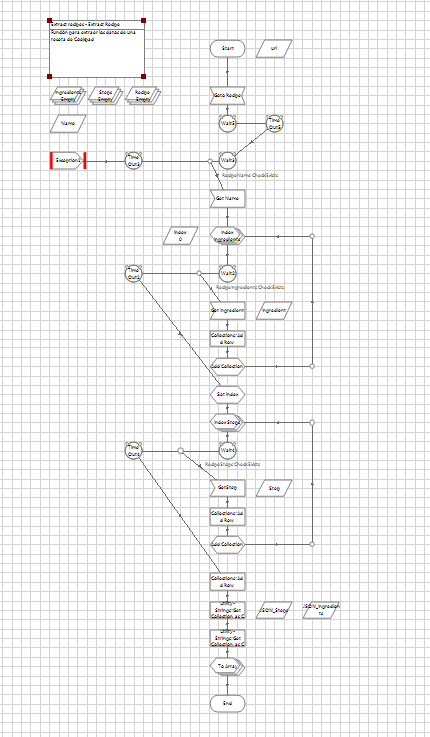
\includegraphics[width=100mm,scale=1]{./doc/images/Extract_recipe.png}}
    \caption{Función para extraer enlaces}
    \label{fig:links}
\end{figure}

En el paso de obtención de la receta, se identifica el nombre de la receta. Utilizando la herramienta de modelado de aplicación que trae incorporada BluePrism. Con ella se puede seleccionar el elemento de la página que se desea extraer y automáticamente se extrae información relevante para la identificación como el identificador del elemento, las clases CSS del mismo, su ruta XPATH, etc... El nombre de las recetas como elemento no es único, al ser una lista de recetas habrá muchas coincidencias que se quieran extraer. Para ello se utiliza el atributo \emph{match_index}, si se selecciona el primer resultado de la página se obtendría el primer nombre. BluePrism permite recuperar atributos dinámicos, en la función el número de coincidencia itera entre uno y diez para obtener diez recetas de cada tipo. Con la coincidencia del elemento, se extrae el enlace y se guarda en una colección que se pasará a la función para extraer recetas. 

\begin{figure}[h!]
    \centering
    \fbox{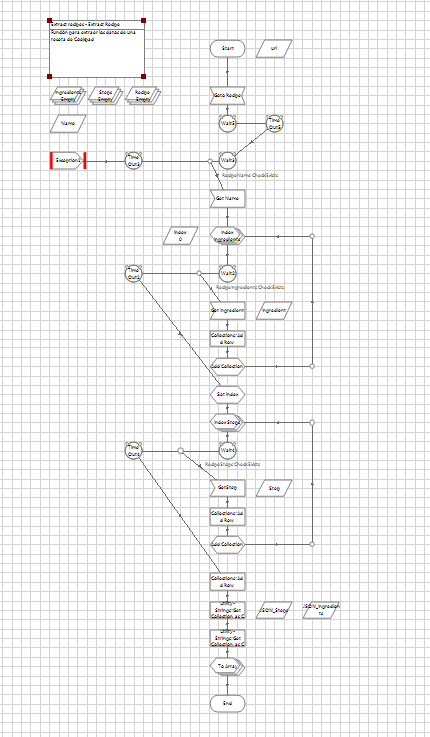
\includegraphics[width=100mm,scale=1]{./doc/images/Extract_recipe.png}}
    \caption{Función para extraer recetas}
    \label{fig:recipe}
\end{figure}

Una vez obtenidos todos los enlaces, puede que haya repetidos por coincidir en la categoría de carne y verduras a la vez, es necesario hacer un filtrado muy sencillo que elimine los enlaces repetidos. 

La función que extrae la receta de la página, obtiene el nombre teniendo en cuenta que es el primer \emph{h1} de la página. Los ingredientes y los pasos se tratan de listas ordenadas, fáciles de extraer. Cada ingrediente tienen un identificador \emph{ingredient} seguido de una cadena de números. BluePrism puede utilizar \emph{wildcards} para identificar elementos de la página web, de la misma manera que al extraer una lista de enlaces, se itera por los ingredientes hasta que no haya más. Con los pasos se sigue el mismo razonamiento, valiéndose de un selector CSS para extraer los pasos iterando sobre ellos hasta que no hay más. 

\begin{figure}[h!]
    \centering
    \fbox{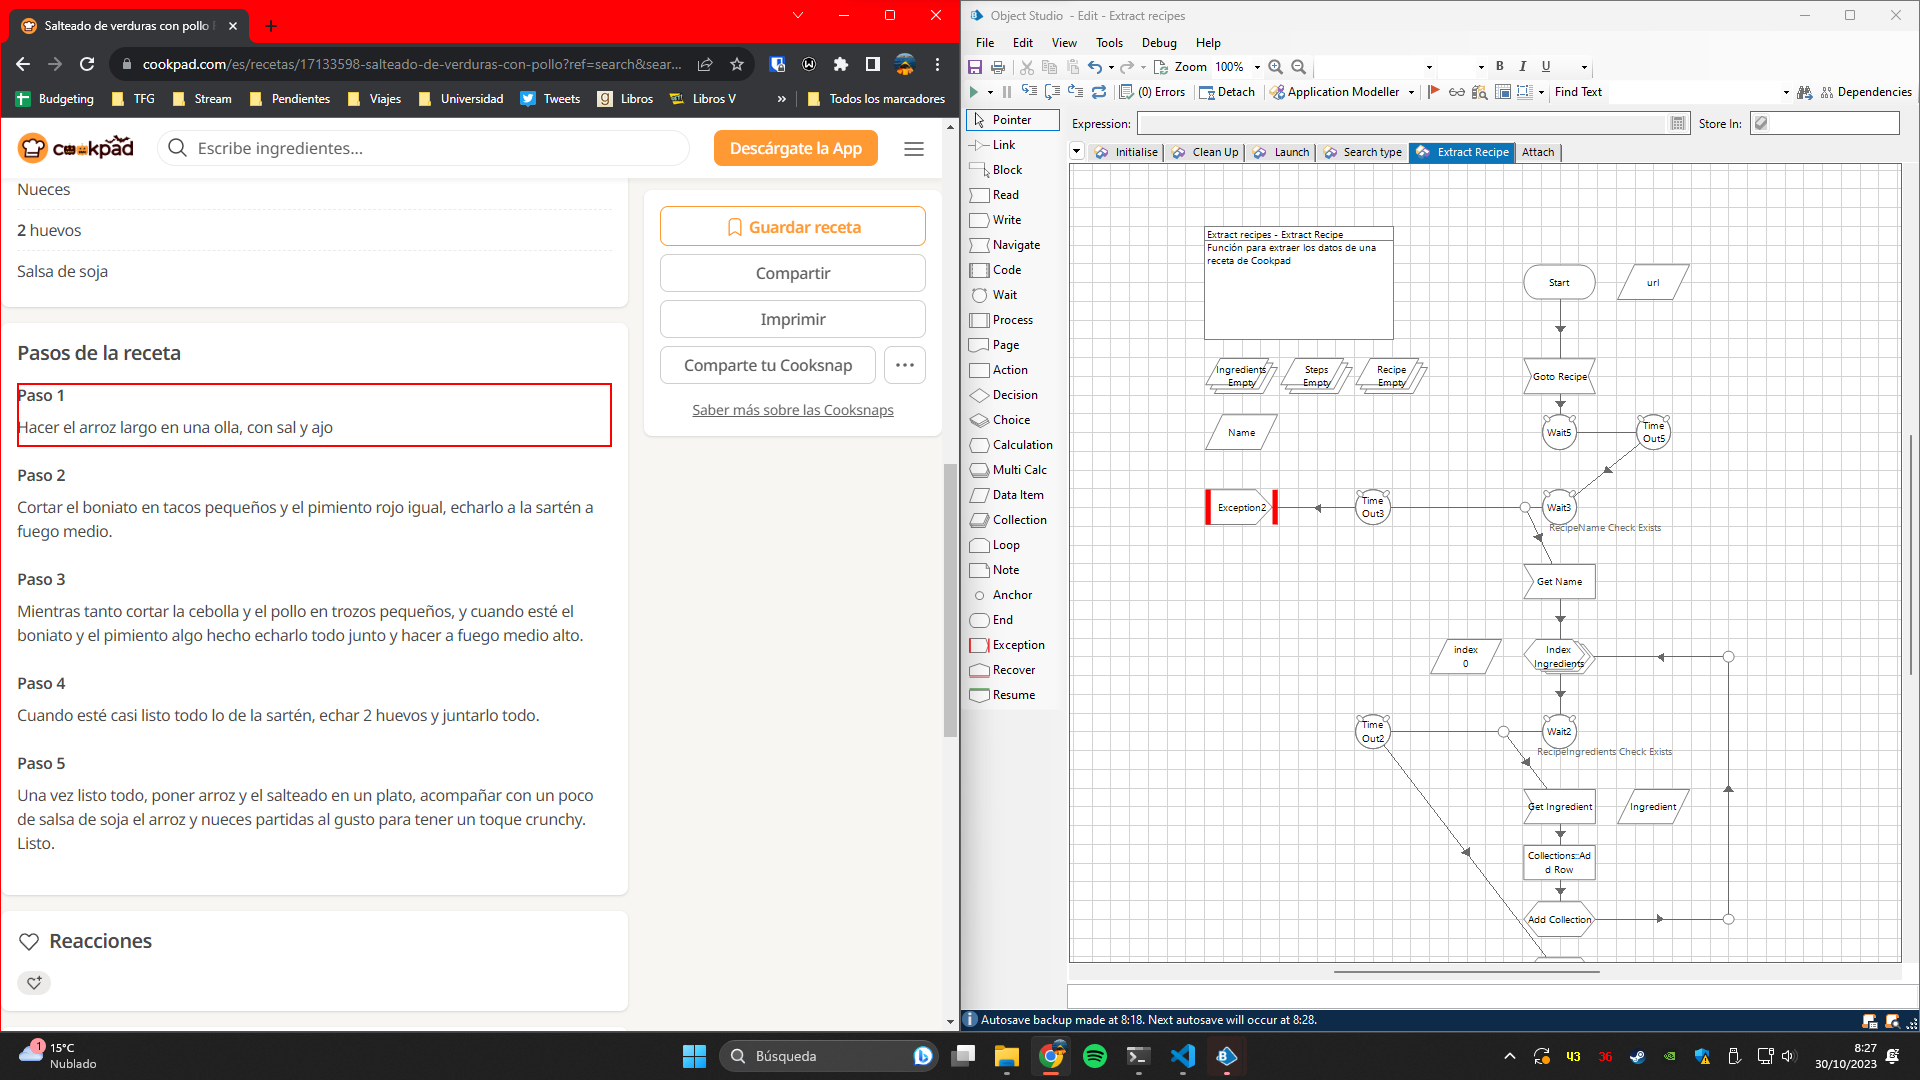
\includegraphics[width=100mm,scale=1]{./doc/images/identify_step.png}}
    \caption{Identificar los pasos de la receta}
    \label{fig:steps}
\end{figure}


Para que constituya una fuente de información uniforme, la colección de recetas se guarda como un fichero JSON que puede ser fácilmente recuperado y transformado en cualquier otro formato.

El proceso de ejecución del robot lleva tiempo, ya que el identificar los ingredientes a través de una expresión regular toma entre diez y veinte segundos. Los demás pasos son relativamente menos costosos en cuestión de tiempo. El robot tardó aproximadamente cuatro horas en obtener sesenta y dos recetas con todos los elementos mencionados. La ventaja de haber utilizado este proceso de obtención de recetas es que se puede ampliar en el futuro a conveniencia, aunque hay que tener en cuenta el tiempo que tarda el robot en obtener recetas.

\section{Gestión de las recetas en la aplicación}

Para insertar los datos en la aplicación, se insertan en una base de datos relacional para aprovechar la relación que existe entre una receta y los ingredientes que contiene. Permitiendo identificar rápidamente que ingredientes lleva una receta, pudiendo gestionar de manera sencilla los requisitos para realizar una receta. 

Se utiliza un pequeño script para insertar los datos desde sus respectivos ficheros a la base de datos siguiendo el siguiente esquema
\begin{figure}[h!]
    \centering
    \fbox{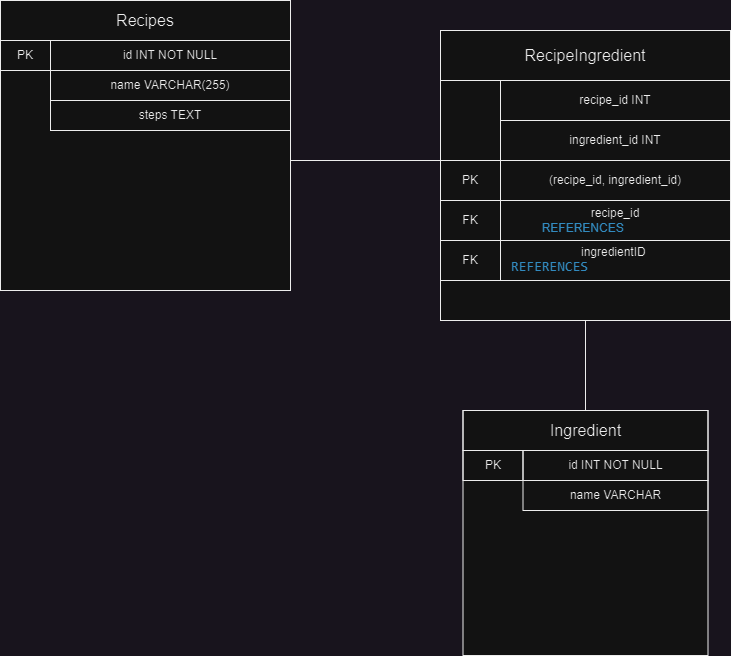
\includegraphics[width=100mm,scale=1]{./doc/images/db.drawio.png}}
    \caption{Esquema de la \gls{base}}
    \label{fig:scheme}
\end{figure}

\section{Encontrar recetas}
El primer problema que se pretende resolver con la publicación del proyecto es permitir a los usuarios encontrar recetas, ya sea por aprovechar los ingredientes de su despensa o porque no recuerdan con exactitud los ingredientes de una receta o sus pasos.


\subsection{Consideraciones iniciales}
Antes de explicar como se ha resuelto el problema debemos hacer unas consideraciones iniciales que se han tomado en cuenta en la etapa de modelización del problema.

Por ejemplo, existen ciertos tipos de ingredientes que todo el mundo tiene en casa, por ello no se consideran como restricciones a la hora de encontrar una receta. Estos son
\begin{enumerate}
    \item Agua
    \item Sal
    \item Pimienta
    \item Aceite
    \item Vinagre
\end{enumerate}

Otra consideración importante es que no se tiene en cuenta la cantidad de cada ingrediente que tiene el usuario en casa. Por ejemplo, puede introducir en el buscador que cuenta con macarrones y tomate frito, obtendrá la receta de ``Macarrones con tomate''. Pero a la hora de cocinar, puede que no tenga pasta suficiente como para una ración completa.

\subsection{Algoritmo}
La funcionalidad se puede implementar de muchas maneras. Quizá la más sencilla sea obtener todas las recetas de la base de datos e ir comprobando una por una las que pueda hacer el usuario con los ingredientes seleccionados. Pero el orden de la función sería  $O(f(n))=n*m$ siendo \textit{n} el número de recetas de la base de datos y m el número de ingredientes que contiene cada una. En este proyecto, al ser una modelización de una solución al problema no se utilizan unos datos demasiado extensos, pero si se extiende el catálogo de recetas la eficiencia se verá afectada gravemente.

Debido a la poca eficiencia en un \gls{dataset} muy grande, es necesario utilizar algunos ajustes previos para reducir lo máximo posible el número de recetas inicial. El primer filtro que se utiliza es el razonamiento de que una receta no será candidata cuando tenga más ingredientes que los seleccionados por el usuario, pues significará que existe un ingrediente que falta. 

Una vez que se ha reducido la búsqueda a un subconjunto de recetas que cuentan con un número de ingredientes menor o igual a los introducidos por el usuario. Existen recetas del subconjunto que no tienen ningún ingrediente de los que se tienen en la despensa, analizar si es una receta candidata será un gasto de tiempo. Del anterior razonamiento nace el segundo filtro aplicado: Obtener solo recetas que contengan al menos un ingrediente de los que ha seleccionado el usuario. 

Al aplicar los dos filtros conjuntamente, se está obteniendo un subconjunto mucho menor y más manejable, solo se necesitaría comprobar que el usuario tenga en su haber los demás ingredientes de la receta.

\subsection{Implementación}
De manera técnica se ha implementado toda la funcionalidad en una misma clase denominada \textit{DB_connector}, que contiene todos los métodos para buscar en la base de datos utilizando diferentes filtros. Además, se han tomado protecciones para que solo haya una clase de este tipo, siendo un \gls{singleton}. Todas las sentencias \gls{SQL} se generan por medio de la herramienta \gls{ORM} utilizando los modelos de las tablas existentes en la base de datos.

La mayoría de métodos son accesos a objetos triviales, con el objetivo de recuperar un objeto por su identificador o por nombre. Se puede ver la información detallada de esta clase en el apéndice de la memoria.

Los dos métodos más relevantes de esta clase son las relativas a buscar recetas: \textit{buscarRecetasNombre}, \textit{buscarRecetasID} y \textit{buscarRecetasIngredientes}.

Al buscar recetas se obtienen también los ingredientes que contienen, con el objetivo de que el usuario pueda comprobar que contiene la receta, o que ingredientes necesitará antes de comprobar los detalles de la misma.

El método para buscar recetas por su nombre, \textit{buscarRecetasNombre}, hace uso de la sentencia \gls{SQL} que selecciona las recetas en base a su nombre, utilizando la función \textit{LIKE},  ignorando las mayúsculas a la hora de buscar la \gls{tupla} en la \gls{base}, devolviendo el identificador y el nombre de las recetas que cumplan la condición.
Para cada receta, se incluyen sus ingredientes, de manera que el usuario tenga en cuenta la posibilidad de que le falte algún ingrediente antes de comprobar los detalles de la receta, iterando los ingredientes que contiene cada receta e introduciéndolos en una lista que será añadida a la \gls{tupla} devuelta.

Por otra parte, \textit{buscarRecetasID}, usa un algoritmo similar a la función anterior. Se recupera la receta de la \gls{base} así como sus ingredientes de manera similar, posteriormente se añade la lista de ingredientes a la \gls{tupla} que será devuelta como resultado de la operación. 

El método \textit{buscarRecetasIngredientes}, utiliza el algoritmo descrito en la sección anterior. Con el método \emph{buscarRecetasIngredientesNumber}, se seleccionan con una sentencia \gls{SQL} todos las las recetas que tengan un número menor de ingredientes que la selección del usuario y tengan al menos un ingrediente de la lista proporcionada. 

Una vez reducido el número de recetas se comprueba si cada ingrediente de la receta está en la lista de ingredientes del usuario. En caso de que no esté, no se debería seguir comprobando esa receta así que se sale del bucle para no perder tiempo. Si la receta cumple, se le añade la lista de ingredientes que se utilizan y a su vez este conjunto se añade al resultado a devolver.
\begin{figure}[H!]
\begin{lstlisting}[style=C, caption={Métodos de la base de datos utilizados para buscar recetas por ingredientes}]
    def buscarRecetasIngredientesNumber(self, id: list[int]):
        try:
            recipes = Recipes.objects.filter(
                Q(number_of_ingredients__lte=len(id)) & Q(recipeingredient__ingredient_id__in=id)
            ).distinct()
            return recipes.all()
        except:
            raise Error_DB("Error de base de datos: No hay conexión con la base de datos")
        
    def buscarRecetasIngredientes(self, id: int):
        try:
            receta_ingredientes = RecipeIngredient.objects.filter(recipe_id=id).values('ingredient_id', ingredient_name=F('ingredient_id__name'))
            resultado = []
            for receta in receta_ingredientes:
                resultado.append((receta['ingredient_id'],receta['ingredient_name']))
            return resultado
        except:
            raise Error_DB("Error de base de datos: No hay conexión con la base de datos")
\end{lstlisting}
    \caption{Clase conector de la \gls{base}}
    \label{cmd:orm}
\end{figure}

\begin{figure}[H!]
    \begin{lstlisting}[style=C, caption={Método del buscador para buscar recetas por ingredientes}]
        try:
            resultados =  self._db.buscarRecetasIngredientesNumber(IDs)
        except:
            raise Error_Buscador("Error Buscador: La sentencia de buscar recetas por id de ingredientes no es correcta")
        try:
            recetas = []
            if resultados:
                for item in resultados:
                    cumple = True
                    lista_ingredientes = []
                    resultados = self._db.buscarRecetasIngredientes(item.id)
                    for resultado in resultados:
                        if not (resultado[0] in IDs):
                            cumple = False
                            break
                        lista_ingredientes.append(resultado[1])
                    if cumple:
                        recetas.append((item.id,item.name,lista_ingredientes))
            return recetas
        except:
            raise Error_Buscador("Error Buscador: La sentencia de buscar ingredientes por id de la receta no es correcta")
    \end{lstlisting}
        \caption{Clase buscador de la aplicación}
        \label{cmd:buscador}
    \end{figure}


\subsection{Tests}
Para una correcta metodología, es necesario contar con una serie de test unitarios que permitan comprobar cada vez que se añade una nueva funcionalidad, la correcta integración de la misma. Como se mencionó en el capítulo de implementación, en el proyecto actual solo existe una funcionalidad, pero se deja la puerta abierta para el desarrollo de nuevas utilidades en el futuro, como añadir cualquier restricción alimentaria que pueda tener el usuario, cambiando los ingredientes problemáticos por unos permitidos para el usuario. 

En el desarrollo de las pruebas se ha realizado con la herramienta pytest. Se ha generado un \gls{test} para cada filtro de la base de datos.
\begin{enumerate}
    \item Recetas
    \begin{itemize}
        \item Identificador
        \item Nombre
        \item Ingredientes
    \end{itemize}
    \item Ingredientes
    \begin{itemize}
        \item Identificador
        \item Nombre
    \end{itemize}
\end{enumerate}

Los test se han añadido en un fichero de python ``test/test.py'' del que se obtienen las pruebas para la integración de la aplicación.
\begin{figure}[h!]
    \centering
    \fbox{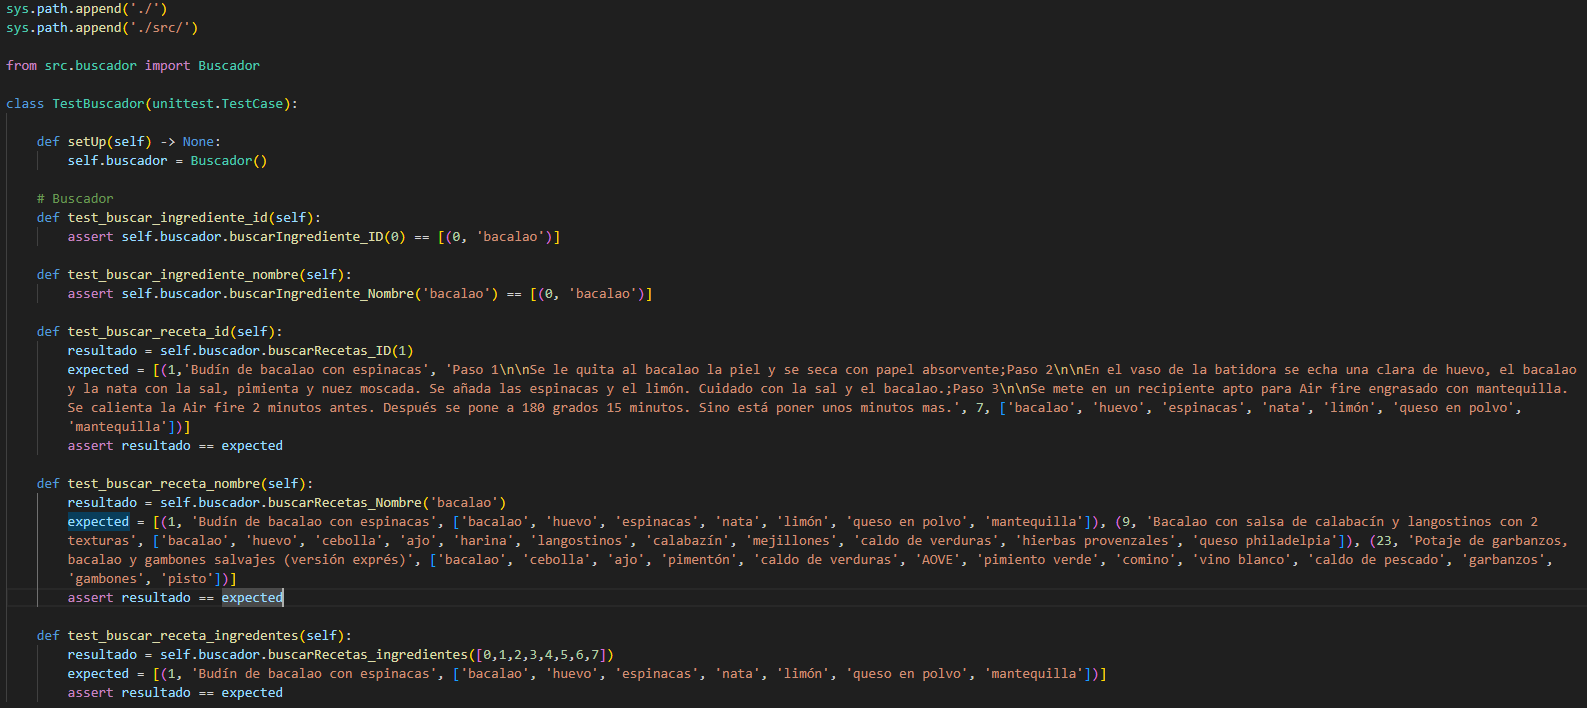
\includegraphics[width=100mm,scale=1]{./doc/images/tests.png}}
    \caption{Clase para testear la funcionalidad buscador}
    \label{fig:test}
\end{figure}

Para ejecutar los test se hace uso de Invoke, el gestor de tareas seleccionado en el proyecto, el código de las pruebas se incluye en el anexo de la documentación. 

\begin{figure}
    \centering
    \begin{lstlisting}[style=consola]
        invoke test
    \end{lstlisting}
    \caption{Comando para lanzar los test unitarios}
    \label{cmd:test}
\end{figure}